\documentclass[pdflatex,sn-apa]{sn-jnl}% APA Reference Style

\usepackage{graphicx}%
\usepackage{multirow}%
\usepackage{amsmath,amssymb,amsfonts}%
\usepackage[title]{appendix}%
\usepackage{xcolor}%
\usepackage{textcomp}%
\usepackage{booktabs}%
\usepackage{array}%
\usepackage{url}%
\usepackage{longtable}%
\usepackage{float}%
\usepackage{placeins}%

\raggedbottom

% Number everything with an S- prefix, standard practice for supplementary
% material accompanying a paper.
\renewcommand{\thesection}{S\arabic{section}}
\renewcommand{\thetable}{S\arabic{table}}
\renewcommand{\thefigure}{S\arabic{figure}}
\renewcommand{\theequation}{S\arabic{equation}}

\begin{document}

\title[Supplementary Material]
{Supplementary Material for: Pitch, Prediction, and Speaker Confounds in U.S.\ Presidential Debates, 1988-2020}

\author*[1]{\fnm{Lavanya} \sur{Prahallad}}\email{lavanya.prahallad@research.iiit.ac.in}

\affil*[1]{\orgdiv{LTRC}, \orgname{IIIT Hyd}, \orgaddress{\street{Gachibowli}, \city{Hyderabad}, \postcode{500032}, \state{Telangana}, \country{India}}}

\abstract{This document is the full supplementary material for the paper
above: the debate inventory, alignment and preprocessing detail, complete
feature definitions, full statistical results, the discourse-annotation
audit, supplementary multimodal models, LLM methods and reproducibility
specification, the exploratory same-candidate analysis, and known corpus
issues. The main paper's appendix gives a short summary of each section
and points here for the full content. Section and table numbers here are
independent of the main paper's numbering (prefixed S).

Code and data are available at:
\url{https://github.com/researchsparkhub/us-presidential-debate-pitch-confounds}}

\maketitle

\section{Debate Inventory}
\label{s:inventory}

\scriptsize
\setlength{\tabcolsep}{2pt}

\begin{longtable}{
@{}
l
l
>{\raggedright\arraybackslash}p{0.42\columnwidth}
l
@{}
}

\caption{Every debate in the corpus: date, candidates, and which ticket won
the election that followed.}
\label{s:tab:inventory}\\

\toprule
\textbf{ID} & \textbf{Date} & \textbf{Candidates} & \textbf{Winner} \\
\midrule
\endfirsthead

\multicolumn{4}{l}{\textit{Table \thetable\ continued}}\\
\toprule
\textbf{ID} & \textbf{Date} & \textbf{Candidates} & \textbf{Winner} \\
\midrule
\endhead

\midrule
\multicolumn{4}{r}{\textit{Continued on next page}}\\
\endfoot

\bottomrule
\endlastfoot
1001 & 1988-09-25 & G.\,H.\,W.\ Bush vs.\ Dukakis & Bush \\
1003 & 1988-10-13 & G.\,H.\,W.\ Bush vs.\ Dukakis & Bush \\
1004 & 1992-10-11 & Clinton vs.\ Perot, G.\,H.\,W.\ Bush & Clinton \\
1006 & 1992-10-15 & Clinton vs.\ Perot, G.\,H.\,W.\ Bush & Clinton \\
1007 & 1992-10-19 & Clinton vs.\ G.\,H.\,W.\ Bush, Perot & Clinton \\
1008 & 1996-10-06 & Clinton vs.\ Dole & Clinton \\
1010 & 1996-10-16 & Clinton vs.\ Dole & Clinton \\
1011 & 2000-10-03 & G.\,W.\ Bush vs.\ Gore & Bush \\
1013 & 2000-10-11 & G.\,W.\ Bush vs.\ Gore & Bush \\
1014 & 2000-10-17 & G.\,W.\ Bush vs.\ Gore & Bush \\
1015 & 2004-09-30 & G.\,W.\ Bush vs.\ Kerry & Bush \\
1017 & 2004-10-08 & G.\,W.\ Bush vs.\ Kerry & Bush \\
1018 & 2004-10-13 & G.\,W.\ Bush vs.\ Kerry & Bush \\
1019 & 2008-09-26 & Obama vs.\ McCain & Obama \\
1021 & 2008-10-07 & Obama vs.\ McCain & Obama \\
1022 & 2008-10-15 & Obama vs.\ McCain & Obama \\
1023 & 2012-10-03 & Obama vs.\ Romney & Obama \\
1025 & 2012-10-16 & Obama vs.\ Romney & Obama \\
1026 & 2012-10-22 & Obama vs.\ Romney & Obama \\
1027 & 2016-09-26 & Trump vs.\ H.\ Clinton & Trump \\
1029 & 2016-10-09 & Trump vs.\ H.\ Clinton & Trump \\
1030 & 2016-10-19 & Trump vs.\ H.\ Clinton & Trump \\
1031 & 2020-09-29 & Biden vs.\ Trump & Biden \\
1033 & 2020-10-22 & Biden vs.\ Trump & Biden \\
\bottomrule
\end{longtable}

\normalsize

\section{Alignment and Preprocessing}
\label{s:align}

Audio was converted to single-channel PCM at $16$~kHz. For matching, both the
recognised text and the official transcript were reduced to lower-case
alphanumeric tokens. Punctuation was removed, contractions were left
unexpanded, and numerals were kept as written. The match rate is the share
of official-transcript tokens that fall inside a matching block. Matching
blocks were found with a longest-matching-block algorithm. Routing
thresholds were $\geq 85\%$ and $60$-$85\%$.

Recognition used Whisper \citep{radford2023whisper}, which gives word-level
timings. Matched tokens take those timings directly. Unmatched runs are
interpolated between the nearest matched words, split by character count.

Montreal Forced Aligner \citep{mcauliffe2017mfa} was run with the English ARPA
acoustic model and dictionary. Default beam settings did not finish on
ninety-minute recordings, so production runs used wider beams under a
watchdog. It converged on $20$ of $24$ debates and is kept as an independent
check.

\section{Complete Feature Definitions}
\label{s:features}

Pitch, loudness and voice-quality measures come from Praat
\citep{boersma2024praat} through \texttt{parselmouth}. The $88$-parameter set
comes from openSMILE \citep{eyben2010opensmile,eyben2016gemaps}, which also
supplies the semitone pitch measures and the second voice-clarity
implementation. Parsing and tagging use spaCy \citep{honnibal2020spacy} with
\texttt{en\_core\_web\_sm}, the smallest available model. Its weakest
outputs are parse depth and dependency length. Sentiment uses VADER
\citep{hutto2014vader}, topic categories use Empath \citep{fast2016empath}, and
sentence vectors use Sentence-BERT \citep{reimers2019sbert}.

A silent pause is a stretch of at least $150$~ms during which loudness stays
at least $25$~dB below the ninetieth percentile for that sentence. The usual
threshold after \citet{goldman1968psycholinguistics} is
$250$~ms. The detector cannot see filled pauses. Whether those were
transcribed at all varies across this corpus.

Table~\ref{s:tab:featuredict} names the $34$ standardized measures used in
the combined multimodal models and the LLM protocol. These overlap heavily
with the full $43$-measure broad screen. The remaining measures are named
individually in the main paper's results: jitter, shimmer, four readability
scores, positive/negative sentiment, and the $35$ topic categories, which
are treated as one diagnostic family rather than as individual screened
measures.

\begin{table}[!htbp]
\caption{The $34$ standardized measures used in the combined and LLM
analyses, by family.}
\label{s:tab:featuredict}
\centering
\scriptsize
\setlength{\tabcolsep}{2pt}
\begin{tabular}{p{0.30\columnwidth}p{0.30\columnwidth}p{0.30\columnwidth}}
\toprule
Acoustic (Praat) & Acoustic (openSMILE) & Linguistic \\
\midrule
Mean pitch & Syllable rate & Clauses \\
Pitch SD (Hz) & Articulation rate (syll/s) & Subordinate clauses \\
Pitch range (Hz) & Semitone pitch SD/mean & Parse depth \\
Loudness & Semitone $20$-$80$ range & Dependency length \\
Voice clarity (Praat) & Voice clarity (openSMILE) & Words per sentence \\
Pause duration & & Word length \\
Pause count & & Function words \\
Mean pause length & & 1st/2nd/3rd-person pronouns \\
Speech rate & & Nouns, verbs, adjectives, adverbs \\
Articulation rate (w/s) & & Reading ease, grade level \\
 & & Sentiment, positive, negative \\
\bottomrule
\end{tabular}
\end{table}

For the frame-level pitch-contour measures, the low-level-descriptor output
of openSMILE (\texttt{F0semitoneFrom27.5Hz\_sma3nz}, $10$~ms hop) was run
independently per sentence clip. We first tried slicing these measures from
a continuously smoothed whole-debate stream, but rejected this approach:
continuous smoothing across sentence boundaries shifted the resulting
statistics measurably at clip edges. Distributional measures use all
voiced frames regardless of order. Dynamic measures use only differences
between temporally consecutive voiced frames. Declination slope and its
residual standard deviation come from an ordinary-least-squares fit of the
semitone contour against frame time.

Four measurement problems are recorded for anyone reusing the corpus.
\emph{One pitch range for everyone}: the analysis range was $75$-$500$~Hz
for a corpus where average pitch runs from $102.5$ to $195.9$~Hz. The
fixed $75$~Hz floor is the likely cause of the pitch-dependence of voice
clarity. \emph{Mismatched floors}: Praat's loudness default assumes a
minimum pitch of $100$~Hz against the $75$~Hz used for pitch. \emph{Voiced
fraction} runs from $0.583$ to $0.742$ across speakers. It correlates with
voice clarity at $+0.674$ at speaker level, and this relationship persists
within a single speaker in a single debate, at a median of $+0.327$.
\emph{Reliability depends steeply on sentence length} (Table~\ref{s:tab:reliab}).

\begin{table}[!htbp]
\caption{Voice-clarity reliability by sentence length. Split-half reliability
is odd-versus-even sentences within one speaker in one debate.}
\label{s:tab:reliab}
\centering
\begin{tabular}{lrrr}
\toprule
Sentence length & Mean clarity & SD & Split-half \\
\midrule
$0.3$-$1.0$~s  & $8.79$~dB  & $3.10$ & $0.126$ \\
$1.0$-$2.5$~s  & $9.51$~dB  & $2.42$ & $0.476$ \\
$2.5$-$6.0$~s  & $9.96$~dB  & $2.16$ & $0.655$ \\
$6.0$~s$+$      & $10.30$~dB & $2.00$ & $0.729$ \\
\midrule
\multicolumn{4}{l}{Candidate sentences: median $3.02$~s, IQR} \\
\multicolumn{4}{l}{$(1.53, 5.71)$; $24.2\%$ under $1.5$~s, $13.1\%$} \\
\multicolumn{4}{l}{under $1.0$~s, $4.6\%$ under $0.5$~s.} \\
\bottomrule
\end{tabular}
\end{table}

\section{Full Statistical Results}
\label{s:stats}

Debate effects are removed by subtracting each debate's mean. Cluster-robust
variances use a sandwich estimator with a small-sample correction. These are
referred to a $t$ distribution with $G-1$ degrees of freedom: $G = 24$ for
debate clustering and $14$ for speaker clustering. With this few clusters
the $p$-values should be read as generous rather than exact.

The randomization test enumerates all $2^{24} = 16{,}777{,}216$ ways of
flipping the winner label within debates. Random-effects pooling follows
DerSimonian-Laird. The prediction interval is computed as the pooled
estimate $\pm\, t_{22}\sqrt{\tau^2 + \mathrm{SE}^2}$. Leave-one-speaker-out
recomputes the within-debate effect with one speaker's sentences removed.

Several of the $43$ measures overlap: $13$ pairs correlate above $|r| =
0.7$. The effective number of independent measures is $30.0$ by the Li-Ji
method. Correcting at $m = 30$ instead of $m = 43$ changes nothing.

The area under the curve (AUC) reported for the discriminant and forest in
the main paper has a direct reading: take one sentence from a winning
candidate and one from a non-winning candidate at random, and AUC is the
probability the model scores the winning one higher. $0.5$ is the right
baseline only when the held-out items are independent.

\section{Discourse Annotation}
\label{s:tagging}

The rule-based labeller assigns dialogue acts and rhetorical categories from
sentence type, word and pattern matches, question syntax, and first-person
stance markers. Two of its categories are copies of the sentence-type column
rather than independent detectors. It returns zero for $13$ codes.
Table~\ref{s:tab:regex} shows what fraction of each category's hits come from
a single string.

\begin{table}[!htbp]
\caption{What the rule-based detectors actually fire on. ``Sole trigger'' is
the share of hits produced by one string and nothing else. ``Rep.'' is the
count after fixing the rule. ``Eff.'' is the difference after fixing.}
\label{s:tab:regex}
\centering
\footnotesize
\setlength{\tabcolsep}{2pt}
\begin{tabular}{lrlrrr}
\toprule
Category & Hits & Sole trigger & Rep. & Eff. & dir. \\
\midrule
Unity framing     & 396   & ``United States'' $80.1\%$ & 69  & $-0.004$ & $10/24$ \\
Patriotic appeal  & 1{,}235 & ``America'' $88.0\%$     & 115 & $-0.014$ & $13/24$ \\
Historical ref.   & 265   & bare year $63.4\%$         & 165 & $-0.028$ & $15/24$ \\
Fear appeal       & 540   & substring $30.9\%$         & 373 & $+0.007$ & $11/24$ \\
Emotional appeal  & 435   & ``children''$+$``families'' & -- & -- & -- \\
Agreement         & 237   & ``absolutely''/``exactly'' & -- & -- & -- \\
Rejection         & 178   & initial ``no'' $93.8\%$    & -- & -- & -- \\
Statement         & 22{,}629 & $=$ declarative $100\%$ & -- & -- & -- \\
Imperative        & 697 & $=$ imperative form $100\%$  & -- & -- & -- \\
\bottomrule
\end{tabular}
\end{table}

Fixing the four fixable rules--anchoring at word boundaries and requiring a
real unity or patriotic phrase--cuts unity framing from $396$ hits to $69$.
It also cuts patriotic appeal from $1{,}235$ to $115$. Between $94$ and $97$
per cent of what these categories counted was something else. What survives
appears in $0.3$ to $0.5\%$ of sentences with differences no larger than
$0.014$.

The corpus was also labelled by a large language model through a batch API,
using a prompt that assigns dialogue acts first and rhetorical categories
second. The model returned a parseable answer for $100.0\%$ of sentences. It
assigned at least one dialogue act to $99.86\%$ of candidate sentences and
at least one rhetorical category to $71.05\%$. Table~\ref{s:tab:kappa} gives
category-level agreement. The two labellings agree best on categories
readable from the grammar (questions, thanks), and worst on the
interpretive ones.

\begin{table}[!htbp]
\caption{Agreement between the rule-based and model labels over $24{,}193$
candidate sentences. PSA (percent specific agreement) treats neither as
the reference. PABAK and AC1 correct for how rare each category is.}
\label{s:tab:kappa}
\centering
\footnotesize
\setlength{\tabcolsep}{3pt}
\begin{tabular}{lrrrrrr}
\toprule
Category & Rule & Model & PSA & $\kappa$ & PABAK & AC1 \\
\midrule
Thanks            & 182   & 217   & $0.852$ & $0.851$ & $0.995$ & $0.998$ \\
Wh-question       & 212   & 376   & $0.599$ & $0.594$ & $0.980$ & $0.990$ \\
Polar question    & 146   & 290   & $0.564$ & $0.561$ & $0.984$ & $0.992$ \\
Explanation       & 1{,}478 & 869 & $0.415$ & $0.387$ & $0.886$ & $0.937$ \\
Personal stance   & 1{,}424 & 4{,}865 & $0.389$ & $0.327$ & $0.682$ & $0.795$ \\
Fear appeal       & 540   & 1{,}674 & $0.237$ & $0.210$ & $0.860$ & $0.923$ \\
Historical ref.   & 265   & 1{,}343 & $0.208$ & $0.193$ & $0.895$ & $0.944$ \\
Patriotic appeal  & 1{,}235 & 282  & $0.190$ & $0.174$ & $0.898$ & $0.946$ \\
Imperative        & 697   & 1{,}234 & $0.177$ & $0.146$ & $0.869$ & $0.929$ \\
Unity framing     & 396   & 1{,}099 & $0.060$ & $0.037$ & $0.884$ & $0.938$ \\
Rebuttal          & 3     & 4{,}653 & $0.001$ & $0.001$ & $0.616$ & $0.767$ \\
Informative stmt. & 2{,}475 & 0    & $0.000$ & $0.000$ & $0.795$ & $0.887$ \\
\midrule
\multicolumn{7}{l}{Whole-set agreement (Krippendorff $\alpha$, MASI):} \\
\multicolumn{7}{l}{dialogue acts $+0.199$; rhetorical categories $+0.012$.} \\
\bottomrule
\end{tabular}
\end{table}

\emph{Chain-of-thought variant.} A natural objection to the direct prompt
above is that it never gives the model room to reason. It goes straight
from sentence to codes. We re-ran the labelling on a stratified sample of
$3{,}001$ candidate sentences ($12.4\%$ of the corpus, proportional across
all $24$ debates), with one change: the output schema requires a short
free-text \texttt{reasoning} field, written before the \texttt{damsl} and
\texttt{beads} codes. This means the model must commit to an explanation
before it commits to a label. It is the same chain-of-thought design that
\citet{wei2022chain} showed can improve accuracy on tasks with a checkable
right answer. The model, codebook, and prompt were otherwise the same
(Section~\ref{s:llmrepro}). It does not help. Figure~\ref{s:fig:cot} gives
Krippendorff's $\alpha$ against the rule tagger for both prompting styles,
recomputed on the identical sample. Dialogue acts move from $+0.167$ direct
to $+0.169$ with reasoning. Rhetorical categories move from $-0.030$ to
$-0.002$. Both changes are within sampling noise of each other, and both
are the same chance-level result as the full-corpus comparison above.
Chain-of-thought and direct prompting agree with \emph{each other} at
$\alpha = +0.564$ for dialogue acts and $+0.536$ for rhetorical categories.
This is moderate agreement, well short of the near-unanimity two runs of a
deterministic rule tagger would show. Both prompting styles remain equally
uncorrelated with the rule-based labels. Reasoning also makes the model
slightly more conservative: it assigns a dialogue act to $98.20\%$ of the
sample and a rhetorical category to $66.61\%$, against $99.83\%$ and
$70.68\%$ for direct prompting on the identical sample. The instrument's
problem was never that the model failed to explain itself. The problem is
that the categories it is asked to detect are not observable from either
the grammar or an explanation. Asking for one does not manufacture the
signal.

\begin{figure}[h]
  \centering
  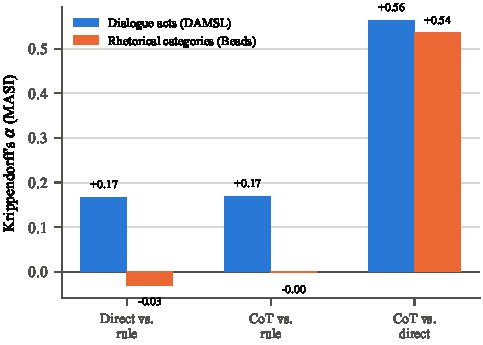
\includegraphics[width=\columnwidth]{fig_cot.pdf}
  \caption{Chain-of-thought prompting does not close the gap with the
  rule-based tagger. Both prompting styles land at the same chance-level
  agreement with the rules; what changes is how much the two LLM conditions
  agree with each other.}
  \label{s:fig:cot}
\end{figure}

\section{Supplementary Multimodal Models}
\label{s:supplement}

\emph{Weighted sum.} Each measure gets a weight equal to how well it
separates the groups in training debates $T$:
\begin{equation}
w_j \;=\; \frac{1}{|W_T|}\sum_{i \in W_T} z_{ij} \;-\;
          \frac{1}{|L_T|}\sum_{i \in L_T} z_{ij} \,,
\label{s:eq:weights}
\end{equation}
The weight vector is scaled to unit length. Each sentence is then scored
as $S_i = \sum_{j=1}^{34} w_j z_{ij}$. Weights are learned on $23$ debates
and scored on the twenty-fourth, rotating through all of them.

\begin{table}[!htbp]
\caption{Combining measures, against the two measures that survived on their
own.}
\label{s:tab:combine}
\centering
\scriptsize
\setlength{\tabcolsep}{2.5pt}
\begin{tabular}{lrrrr}
\toprule
 & \multicolumn{2}{c}{Single measures} & \multicolumn{2}{c}{Composite (34 measures)} \\
\cmidrule(lr){2-3}\cmidrule(lr){4-5}
 & Semitone & Semitone & hold out & hold out \\
 & 20-80 range & SD/mean & debate & speakers \\
\midrule
Mean per-debate effect & $-0.243$ & $\mathbf{-0.370}$ & $+0.390$ & $+0.070$ \\
SD across debates      & $0.289$  & $0.358$  & $0.603$ & $0.519$ \\
Debates in direction   & $21/24$  & $20/24$  & $17/24$ & $11/24$ \\
Sign-test $p$          & $0.0003$ & $0.0015$ & $0.064$ & $0.84$ \\
\bottomrule
\end{tabular}
\end{table}

On held-out debates, the weighted composite reaches $+0.390$ standard
deviations, a $60\%$ improvement on the semitone percentile range alone.
But it is markedly less consistent (SD across debates $0.603$ against
$0.289$). Under speaker holdout it falls to $+0.070$. A single measure
needing no training is more reliable than a weighted combination of $34$.

\emph{Discriminant loadings.} Averaged to the $51$ speaker-by-debate cells,
the discriminant separates winning from non-winning cells at an area under
the curve of $0.907$. Table~\ref{s:tab:loadings} reports the correlation
between each measure and the discriminant score. Correlations are more
stable than raw weights when measures are correlated.

\begin{table}[!htbp]
\caption{What the discriminant leans on. Positive means higher among winning
candidates.}
\label{s:tab:loadings}
\centering
\footnotesize
\begin{tabular}{lr}
\toprule
Measure & Loading \\
\midrule
Voice clarity (openSMILE)       & $+0.628$ \\
Semitone pitch SD/mean          & $-0.587$ \\
Voice clarity (Praat)           & $+0.462$ \\
Pitch SD (Hz)                   & $-0.422$ \\
Semitone $20$-$80$ pitch range & $-0.410$ \\
Pitch range (Hz)                & $-0.317$ \\
Articulation rate (syll/s)      & $+0.235$ \\
Mean pitch                      & $+0.189$ \\
Pause duration                  & $+0.186$ \\
Articulation rate (words/s)     & $+0.181$ \\
\bottomrule
\end{tabular}
\end{table}

Every measure in the top ten is acoustic. Nothing syntactic, lexical or
semantic appears until well below. The highest-loading measure is the one
shown in the main paper to track the speaker's own pitch at $r = +0.78$ to
$+0.90$. Consistent with that, $81.0\%$ of the variance in the cell scores
is explained by which speaker the cell belongs to.

\emph{Principal component analysis.} PCA asks whether the outcome happens to
line up with the largest-variance directions among the $34$ measures without
using the labels at all.

\begin{figure*}[t]
  \centering
  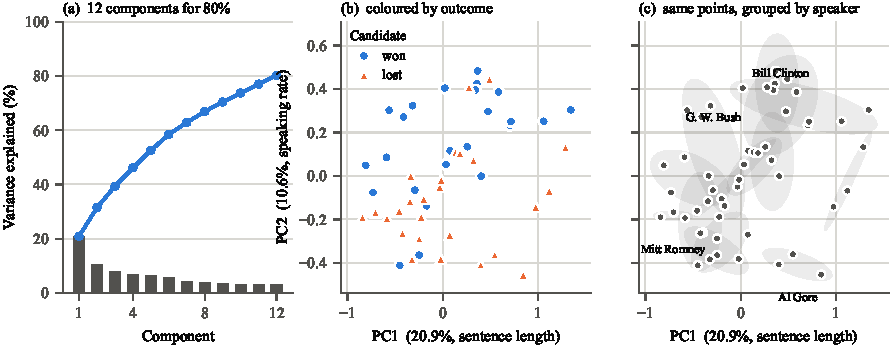
\includegraphics[width=0.99\textwidth]{fig_pca.pdf}
  \caption{Principal component analysis of the $34$ standardized measures.
  (a) Twelve components are needed for $80\%$ of the variance. (b) Each
  point is one candidate in one debate, coloured by outcome. (c) The same
  points, with an ellipse around each speaker's debates. The apparent
  separation by outcome in (b) coincides with the speaker grouping in (c).}
  \label{s:fig:pca}
\end{figure*}

\begin{table}[!htbp]
\caption{Principal components of the $34$ standardized measures.}
\label{s:tab:pca}
\centering
\footnotesize
\setlength{\tabcolsep}{3pt}
\begin{tabular}{lrrl}
\toprule
 & \% of & Separation & Dominant measures \\
 & variance & of groups & \\
\midrule
PC1 & $20.9$ & $+0.006$ & Sentence length, grade level \\
PC2 & $10.6$ & $+0.136$ & Articulation rate, speech rate \\
PC3 & $7.9$  & $+0.203$ & Pitch SD, reading ease \\
PC4 & $6.8$  & $+0.070$ & Mean pitch, voice clarity \\
PC5 & $6.4$  & $+0.359$ & Voice clarity (both tools) \\
PC6 & $5.9$  & $+0.044$ & Sentiment \\
\midrule
\multicolumn{4}{l}{$12$ components needed for $80\%$ of variance.} \\
\multicolumn{4}{l}{At cell level, speaker explains $83.6\%$ of PC1 and} \\
\multicolumn{4}{l}{$86.6\%$ of PC2 positions.} \\
\bottomrule
\end{tabular}
\end{table}

PC1 ($20.9\%$ of variance) is a sentence-length dimension separating the
groups at $+0.006$ standard deviations--nothing. PC2 is speaking rate. The
component that best separates the groups is PC5, at $+0.359$, accounting for
only $6.4\%$ of the variance. A hand-built weighted sum, a supervised
discriminant, and an unsupervised decomposition that ignores the labels
entirely all reach the same place: what structure exists in these $34$
measures is mostly about who is speaking.

\emph{LLM ``both'' condition.} Given the transcript and the descriptor
table together, the model calls $24$ of $24$ debates correctly. This
agrees with the transcript-only condition (main paper) on all $24$
debates. Adding numeric descriptors to a transcript the model can already
place in history changes nothing, because the transcript had already
settled the answer.

\section{LLM Methods and Reproducibility}
\label{s:llmrepro}

This appendix specifies every language-model call in the paper: the original
discourse tagging and its chain-of-thought variant (Section~\ref{s:tagging}),
and the cross-modal winner prediction with its contamination probe. The goal
is that another researcher could reissue every call from this description
alone.

\emph{Model.} All components use the same model, \texttt{claude-opus-4-8},
accessed through Anthropic's Messages API. Anthropic does not publish a
parameter count for this model, so none is reported here. Reporting one
would imply a precision we do not have. Every call uses structured
(\texttt{json\_schema}) output: the model's response is constrained at
generation time to match a schema we specify, rather than parsed after the
fact from free text. All calls were issued on $2026$-$08$-$06$.

\emph{Sampling.} This model deprecates the \texttt{temperature} parameter.
The API rejects a request that sets it. Repeated calls therefore draw on
whatever sampling variability the API applies by default, not on a
caller-chosen temperature. Where the paper reports a repeat count, that is
the only lever available for measuring stability.

\emph{Discourse tagging.} System prompt, codebook and full JSON schema are
reproduced verbatim in \texttt{Sahana Project/tagging\_prompt.md} (direct)
and \texttt{Sahana Project/cot\_tagging\_prompt.md} (chain-of-thought) in
the code repository. Both send $10$ sentences per request, batched for
throughput, with the system prompt and codebook cached
(\texttt{cache\_control: ephemeral}) across requests. The only schema
difference is one field, \texttt{reasoning}, which the chain-of-thought
variant requires before \texttt{damsl} and \texttt{beads}. Structured
output fills schema fields in the order they are declared. This forces the
free-text reasoning to be generated before the codes rather than after
them.

\emph{Cross-modal winner prediction.} System prompt, both JSON schemas
(descriptor-citing and theme-citing), the contamination-probe prompt and
schema, and the closed evidence vocabularies are reproduced verbatim in
\texttt{Sahana Project/crossmodal\_prompt.md} in the code repository. One
call is issued per debate, per condition, per repeat. Each repeat uses a
freshly randomised Candidate-A/B/C letter assignment, shared across
conditions within that repeat so predictions are comparable
trial-for-trial. The contamination probe issues one further call per
debate per input type, with no repeats. It is a single-shot identification
question rather than a graded judgement. Every call uses a fresh, empty
context, so agreement or disagreement between conditions reflects the
input alone.

\emph{Anonymisation.} Candidate names, party affiliation and the debate
date are removed from every input. Moderator turns are dropped entirely,
leaving only candidate sentences in original chronological order. This is
a partial defence at best. A transcript's content--quoted lines, named
policies, the other candidate's real name spoken aloud mid-turn--was not
scrubbed. Removing it would have taken out the communicative content the
transcript condition exists to test. The contamination probe measures what
leaks through this partial anonymisation rather than assuming it is
complete. All $24$ of $24$ transcripts were identified regardless of the
redaction.

\emph{Grounding check.} A cited measure counts as consistent with a
debate's real data when the candidate it names as favoured actually has
the higher within-debate standardized value for that measure. A margin of
less than $0.15$ standard deviations between the two candidates is scored
as ``similar'' and excluded rather than forced to a side. This is an
automatic, closed-vocabulary check, not a human judgement of whether the
reasoning sounds plausible.

\section{Exploratory Same-Candidate Analysis}
\label{s:samecand}

\begin{table}[!htbp]
\centering
\caption{Where the same speaker lands when they won and when they lost.
The discriminant was fitted \emph{without} that speaker, then their debates
were projected in. Scores are relative to the opponent on the night.}
\label{s:tab:within}

\footnotesize
\setlength{\tabcolsep}{5pt}
\renewcommand{\arraystretch}{1.08}

\begin{tabular}{llcr}
\toprule
\textbf{Speaker} & \textbf{Debate} & \textbf{Outcome} & \textbf{Score} \\
\midrule

\multirow{5}{*}{G.\,H.\,W.\ Bush}
 & 1988, first  & won  & $-0.021$ \\
 & 1988, second & won  & $-0.066$ \\
 & 1992, first  & lost & $-0.224$ \\
 & 1992, second & lost & $-0.203$ \\
 & 1992, third  & lost & $-0.223$ \\
\cmidrule(lr){2-4}
 & \multicolumn{2}{l}{Gap (won $-$ lost)} & $+0.173$ \\
 & \multicolumn{2}{l}{Winning above losing} & $6/6$ \\

\midrule

\multirow{5}{*}{Donald Trump}
 & 2016, first  & won  & $+0.010$ \\
 & 2016, second & won  & $-0.018$ \\
 & 2016, third  & won  & $-0.025$ \\
 & 2020, first  & lost & $-0.034$ \\
 & 2020, second & lost & $+0.002$ \\
\cmidrule(lr){2-4}
 & \multicolumn{2}{l}{Gap (won $-$ lost)} & $+0.005$ \\
 & \multicolumn{2}{l}{Winning above losing} & $4/6$ \\

\bottomrule
\end{tabular}
\end{table}
\FloatBarrier

\section{2024 Exclusion and Known Corpus Issues}
\label{s:known}

Two 2024 debates exist in the corpus but are held out, because we could
not verify who was speaking. Their official transcripts are paraphrased
news summaries, sharing only $5.2\%$ and $5.5\%$ of their words with the
audio. As a result, the recognised text was used as the transcript, and
speakers were assigned by diarization \citep{bredin2023pyannote}. That
diarization was never checked against hand-labelled data. We have no
error rate for it.

Four things prompted the exclusion. In the June 2024 debate one candidate is
credited with $786$ sentences and the other with $256$--three to one, in a
format with timed turns and muted microphones. In the September debate about
$285$ sentences sit in twelve or more leftover speaker clusters. Across the
pair, $1{,}162$ sentences are labelled \emph{audience}, in two debates with no
audience. Finally, candidates account for $43.9\%$ of sentences in these
two, against $76$ to $86\%$ everywhere else.

The confirmation is what happens on removal: across the remaining $24$
debates, unattributed sentences drop to zero and audience sentences to $287$.
All of the unattributed material and $80.2\%$ of the audience material came
from those two debates. Including the pair changes several results. Noun
rate flips sign, from $-0.012$ to $+0.043$. Sentiment roughly halves. The
embedding axis rotates (cosine similarity $0.895$ to the one reported
here). Finally, $19$ of the $50$ most extreme sentences at one end come
from this $9.5\%$ of the data. These transcripts also contain no
truncation marks and no filled pauses at all. As a result, interruption
and self-correction are missing by construction.

\subsection*{Availability}
The corpus is deposited as code and derived data at
\url{https://github.com/researchsparkhub/us-presidential-debate-pitch-confounds}.
Released material covers the annotation layers, the per-sentence features
and the checking scripts. Alignment scripts point at audio sourced
elsewhere, which cannot be redistributed; see that repository's
\texttt{DATA\_AVAILABILITY.md} for how to source it.
\label{s:resource}

\bibliography{sn-bibliography}

\end{document}
